\begin{blocksection}
\question
Consider the following FSM. What does it do?

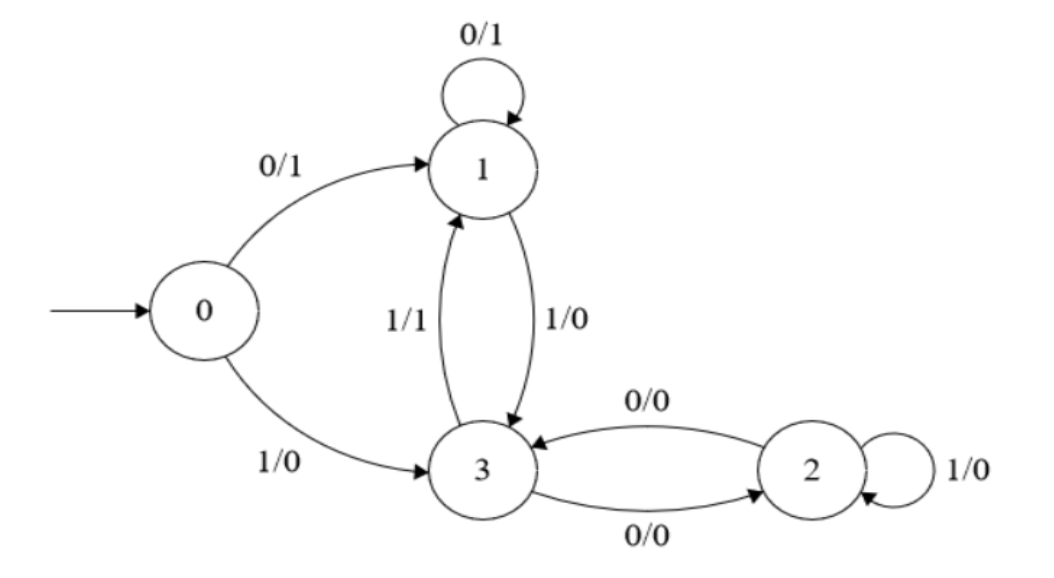
\includegraphics{fsm/basics_4}

\begin{solution}
Meta: This will likely need more scaffolding.
The FSM outputs a 1 whenever the input is a multiple of 3. Some ways to approach analyzing:
\begin{itemize}
\item 1 is a less common output than 0 → what causes a 1 to be output?
\item Trace along the paths → what causes a 0 to be output?
\begin{itemize}
	\item Consider 0,  0,  1 → 0b001 = 1 is not  a multiple of 3
	\item Consider 1, 1 → 0b11 = 3 is a multiple of 3
	\item Consider 1, 1, 1 → 0b111 = 7 is not a multiple of 3
\end{itemize}
\item Brute-force: draw out the truth table
\end{itemize}
\end{solution}

\end{blocksection}